\section{أنواع خوارزميات الملاحقة}
يمكن تصنيف خورازميات الملاحقات بشكل عام كما يلي :

\begin{itemize}
	\item
هل هي قصيرة المدى أم بعيدة المدى
\begin{itemize}
\item
خوارزميات ملاحقة قصيرة المدى
\textLR{short-term trackers}:
مهمتها هي تقدير حالة الغرض
حتى تفشل عملية الملاحقة، وتكون عملية إعادة الملاحقة غير مطلوبة. عادة يتم تقييمها على فيديوهات قصيرة لا تتجاوز 
\textLR{1000}
إطار.
\item
خوارزميات ملاحقة البعيدة المدى 
\textLR{long-term trackers}:
من ضمن أهدافها إعادة الملاحقة في حال الفشل أو في حال اختفاء الغرض من مجال الرؤية. عادة يتم تقييمها على فيديوهات طولها  
\textLR{10000-1000}
		  إطار.
\end{itemize}
\item مسألة ملاحقة بكاميرا واحدة أو عدة كاميرات
\item 
ملاحقة هدف واحد 
\textLR{SOT}
% \selectlanguage{english}
%\begin{figure}[H]
%	\centering
%	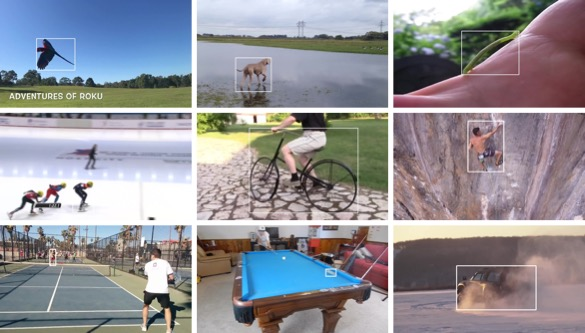
\includegraphics[width=\textwidth]{images/got10k}
%	\caption{
%		VOT
%		\textRL{لأغراض}
%		got10k \cite{got10k}
%		\textRL{عينات من مجموعة معطيات التدريب}
%	}	
%\end{figure}
%\selectlanguage{arabic}
أو
 عدة أهداف
\textLR{MOT}
%\selectlanguage{english}
%\begin{figure}[!h]
% 	\centering
% 	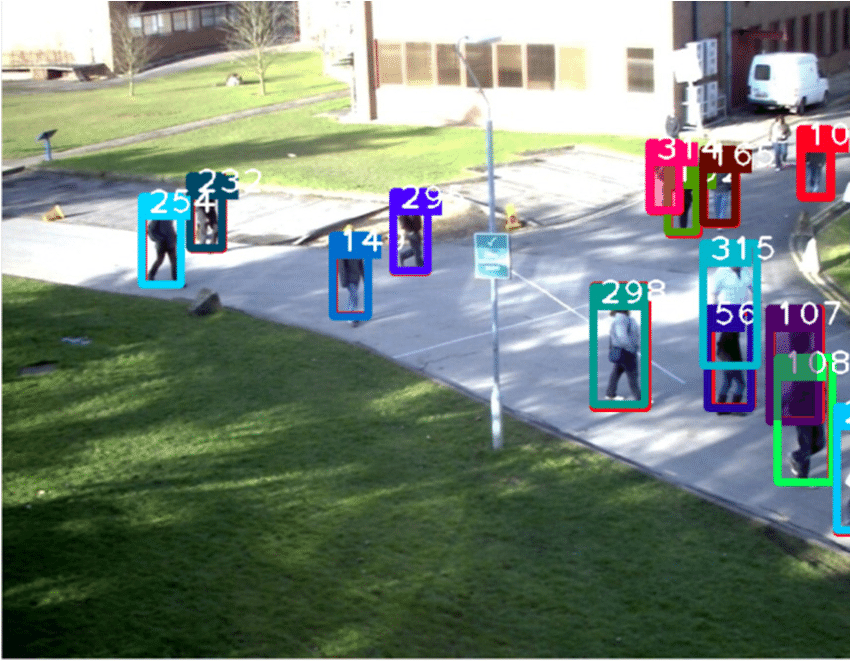
\includegraphics[width=\textwidth]{images/MOT15}
% 	\caption{
%		MOT
%		\textRL{لأغراض}
% 		\cite{Mot15}
% 		Mot15
% 		\textRL{ مثال عن مجموعة معطيات التدريب}
% 	}	
%\end{figure}
%\selectlanguage{arabic}
\item
ملاحقة سببية أو فورية
 \textLR{online tracker}،
غير سببية أو مؤجلة
 \textLR{offline tracker}:
\begin{itemize}
\item
خوارزميات ملاحقة غير سببية:
في بعض التطبيقات  كتحليل الفيديو مثلا، لا نحتاج إلى معرفة مكان الغرض  بشكل لحظي، عندها يمكن معالجة كامل صور  الفيديو دفعة واحدة، إذ يكون التركيز على دقة الملاحقة أكثر  من سرعة عملية المعالجة. وسميت بالملاحقات غير السببية لأن نتيجة الملاحقة لإطار معين يمكن أن تعتمد على الإطارات اللاحقة.
	
\item
خوارزميات ملاحقة سببية:
خرج الملاحقة من أجل الإطار الحالي يعتمد فقط على الإطارات السابقة، وهو الأكثر انتشاراً كون معظم تطبيقات الملاحقة تتطلب الحصول على النتيجة بشكل فوري.
	
\end{itemize}
\end{itemize}
نهتم في بحثنا بخوارزميات الملاحقة السببية، كاميرا واحدة، قصيرة المدى، و بالملاحقة بالزمن الحقيقي.